\chapter{Конструкторский раздел}\label{sec:design}
Раздел содержит описание работы алгоритмов и обоснование структур данных, выбранных при их реализации, оценку используемой памяти и описание системы тестирования программного обеспечения.

\section{Описание структуры ПО}

Программа будет включать в себя один смысловой модуль, назы­ваемый find, который содержит в себе процедуры и функции, связанные с реализацией алгоритмов поиска в словаре по ключу. Независимо от мо­дуля будет существовать файл main.go, реализующий пользовательский интерфейс. Также реализована программа на языке python, которая формирует данные для словаря.

\section{Оценка памяти для хранения данных}

Расчет памяти, используемой для хранения словаря, производится по формуле \ref{math:mem-nonseg}.
\begin{equation}\label{math:mem-nonseg}
M_{dict} = N \cdot (|char| \cdot |key_i| + |int|)
\end{equation}
где $N$ -- количество слов в словаре, $|char|$ -- размер переменной типа <<символ>>, $|key_i|$ -- длина ключа, $|int|$ --  размер переменной типа <<целое>>.
Расчет памяти, используемой под сегментированный массив, вычисляется по формуле \ref{math:mem-seg}.
\begin{equation}\label{math:mem-seg}
M_{seg-dict} = S \cdot M_{dict}
\end{equation}
Где $S$ -- количество сегментов.

\section{Схемы алгоритмов}\label{sec:design-flowcharts}
На рисунке \ref{fig:brute} представлена схема работы алгоритма полного перебора.
\begin{center}
	\begin{figure}[H]
		\centering
		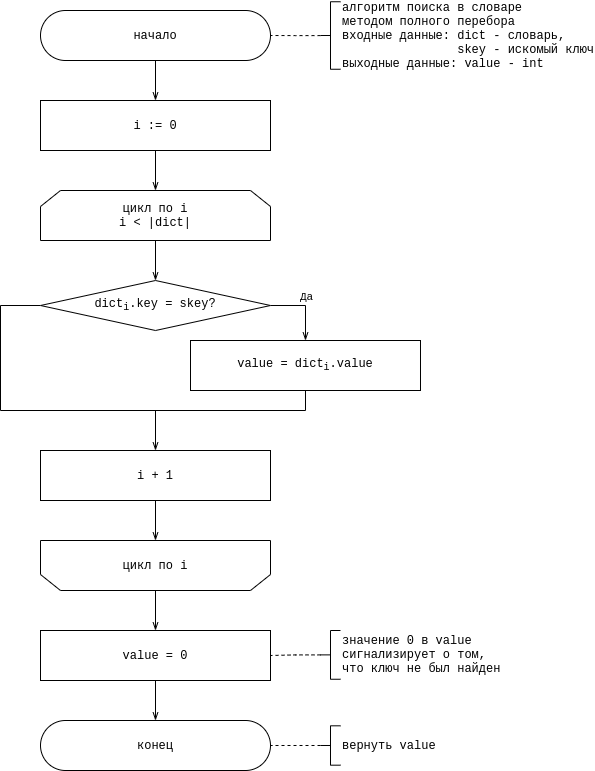
\includegraphics[width=0.83\linewidth]{assets/dict-brute.drawio.png}
		\caption{Схема работы алгоритма полного перебора}
		\label{fig:brute}
	\end{figure}
\end{center}

\begin{center}
	\begin{figure}[H]
		\centering
		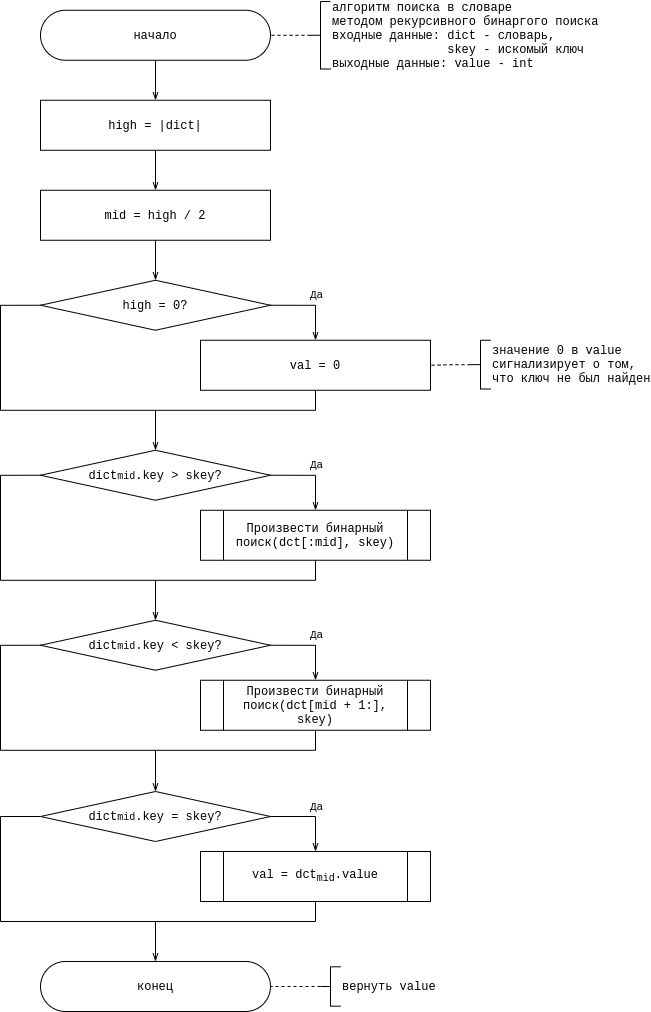
\includegraphics[width=0.83\linewidth]{assets/dict-binary.drawio.png}
		\caption{Схема работы алгоритма бинарного поиска}
		\label{fig:bin}
	\end{figure}
\end{center}

На рисунке \ref{fig:bin} представлена схема работы алгоритма бинарного поиска. Операция взятия среза обозначена как <<$[:]$>>.

\begin{center}
	\begin{figure}[H]
		\centering
		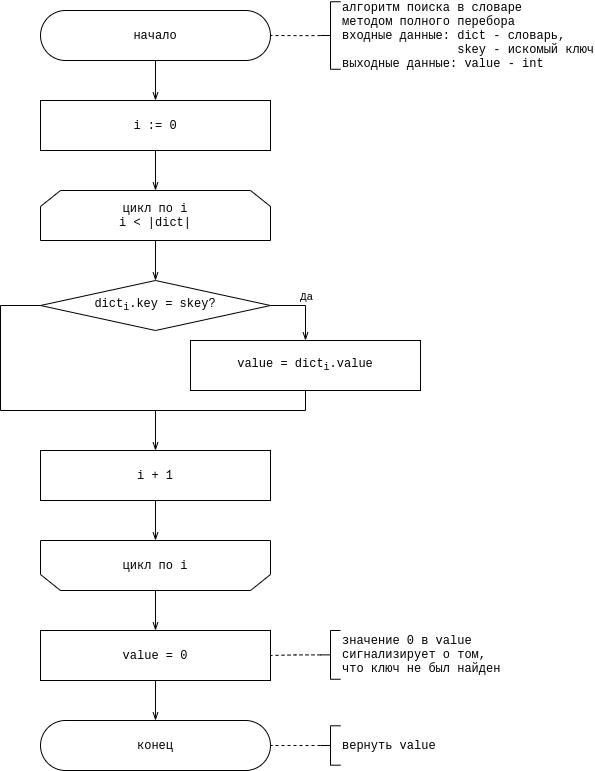
\includegraphics[width=0.95\linewidth]{assets/dict-segment.drawio.png}
		\caption{Схема работы алгоритма бинарного поиска для словаря, поделенного на сегменты}
		\label{fig:seg}
	\end{figure}
\end{center}

На рисунке \ref{fig:seg} представлена схема работы алгоритма бинарного поиска для словаря, поделенного на сегменты. Вызываемая в теле условного оператора функция представлена на рисунке \ref{fig:bin}.

\section{Вывод}

Были разработаны схемы алгоритмов, необходимых для решения задачи. Получено достаточно теоретической информации для написания программного обеспечения.
